\section{Ветвящиеся процессы Гальтона-Ватсона}
\begin{note}
Физическая модель случайного процесса состоит в том, что в дискретные моменты времени частицы распадаются на случайное количество таких же частиц.
\end{note}
\begin{definition}
Пусть $\displaystyle \xi $ -- случайная величина со значениями в $\displaystyle \mathbb{Z}_{+} =\{0,\ 1,\ 2,\dotsc \}$. Пусть $\displaystyle \left\{\xi _{k}^{( n)} ,\ k,\ n\in \mathbb{N}\right\}$ -- независимые одинаково распределенные случайные величины с тем же распределением, что и у $\displaystyle \xi $. Положим $\displaystyle X_{0} =1,\ X_{n} =\sum _{k=1}^{X_{n-1}} \xi _{k}^{( n)} ,\ n\geqslant 1$. Тогда последовательность $\displaystyle ( X_{n} ,\ n\in \mathbb{Z}_{+})$ называется \textit{ветвящимся процессом Гальтона-Ватсона} с законом размножения частиц $\displaystyle \xi $.
\end{definition}
\begin{note}
В модели ветвящегося процесса $\displaystyle X_{n}$ -- число потомков в момент времени $\displaystyle n$, $\displaystyle \xi _{k}^{( n)}$ -- число потомков $\displaystyle k$-ой частицы в $\displaystyle ( n-1)$-ый момент времени.
\end{note}
\begin{definition}
Пусть $\displaystyle \xi $ -- случайная величина. Тогда ее \textit{производящей функцией} называется $\displaystyle \phi _{\xi }( z) =Ez^{\xi }$.
\end{definition}
\begin{proposition}
(Свойства производящей функции, б/д)
\begin{enumerate}
    \item $\displaystyle \phi _{\xi }( 1) =1$.
    \item $\displaystyle \phi _{\xi }^{'}( 1) =E\xi$.
    \item Если $\displaystyle \xi ,\ \eta $ -- независимы, то $\displaystyle \phi _{\xi +\eta }( z) =\phi _{\xi }( z) \cdotp \phi _{\eta }( z)$.
\end{enumerate}
\end{proposition}
\begin{proposition}
(Свойства производящей функции при $\displaystyle \xi \in \mathbb{Z}_{+}$, б/д)
\begin{enumerate}
    \item $\displaystyle \phi _{\xi }( z) =\sum _{k=0}^{\infty } z^{k} P( \xi =k)$ -- степенной ряд, который сходится на множестве $\displaystyle \{| z| \leqslant 1\}$.
    \item В области $\displaystyle \{| z| < 1\}$ функция $\displaystyle \phi _{\xi }( z)$ является аналитической (т.е. совпадает со своим рядом Тейлора в окрестности любой точки области определения) и бесконечно дифференцируемой.
    \item $\displaystyle P( \xi =k) =\dfrac{1}{k!}\left(\dfrac{\partial ^{k}}{\partial z^{k}} \phi _{\xi }( z)\right) \biggr\rvert_{z=0}.$
\end{enumerate}
\end{proposition}
\begin{proposition}
Пусть $\displaystyle ( X_{n} ,\ n\in \mathbb{Z}_{+})$ -- ветвящийся процесс с законом размножения (РАЗЛОЖЕНИЯ?) частиц $\displaystyle \xi $. Тогда, если $\displaystyle z\in [ 0,\ 1]$, то $\displaystyle \phi _{X_{n}}( z) =\phi _{X_{n-1}}( \phi _{\xi }( z))$.
\end{proposition}
\begin{proof}
По определению $\displaystyle \phi _{X_{n}}( z) =Ez^{X_{n}} =E\left( E\left( z^{X_{n}} \ |\ X_{n-1}\right)\right)$. Рассмотрим условное математическое ожидание
\begin{gather*}
E\left( z^{X_{n}} |X_{n-1} =m\right) =E\left( z^{\sum _{k=1}^{X_{n-1}} \xi _{n}^{( k)}} \ |\ X_{n-1} =m\right) =E\left( z^{\sum _{k=1}^{m} \xi _{n}^{( k)}} \ |\ X_{n-1} =m\right) =\\
=\prod _{k=1}^{m} E\left( z^{\xi _{k}^{( n)}} \ |\ X_{n-1} =m\right) =\prod _{k=1}^{m} E\left( z^{\xi _{k}^{( n)}} \ \right) =( \phi _{\xi }( z))^{m} .
\end{gather*}
Тогда $\displaystyle E\left( z^{X_{n}} \ |\ X_{n-1}\right) =( \phi _{\xi }( z))^{X_{n-1}}$, и
\begin{equation*}
\phi _{X_{n}}( z) =E\left(( \phi _{\xi }( z))^{X_{n-1}}\right) =\phi _{X_{n-1}}( \phi _{\xi }( z)) .
\end{equation*}
\end{proof}
\begin{corollary} ~
\begin{enumerate}
    \item $\displaystyle \phi _{X_{n}}( z) =\phi _{\xi }( \phi _{\xi }( \dotsc ( \phi _{\xi }( z)) \dotsc ))$ ($\displaystyle n$ итераций)
    \item $\displaystyle \phi _{X_{n}}( z) =\phi _{\xi }( \phi _{X_{n-1}}( z))$.
\end{enumerate}
\end{corollary}
\begin{proof} ~
\begin{enumerate}
    \item $\displaystyle \phi _{X_{n}}( z) =\phi _{X_{n-1}}( \phi _{\xi }( z)) =\phi _{X_{n-2}}( \phi _{\xi }( \phi _{\xi }( z))) =\dotsc =\phi _{\xi }( \phi _{\xi }( \dotsc ( \phi _{\xi }( z)) \dotsc ))$.
    \item $\displaystyle \phi _{X_{n}}( z) =\phi _{\xi }( \phi _{\xi }( \dotsc ( \phi _{\xi }( z)) \dotsc )) =\phi _{\xi }( \phi _{X_{2}}( \phi _{\xi }( \dotsc ( \phi _{\xi }( z)) \dotsc ))) =\dotsc =\phi _{\xi }( \phi _{X_{n-1}}( z))$.
\end{enumerate}
\end{proof}
\begin{definition}
Пусть $\displaystyle q_{n} =P( X_{n} =0) ,\ q=P( \exists n:\ X_{n} =0)$, где $\displaystyle q$ называется \textit{вероятностью вырождения}.
\end{definition}
\begin{lemma}
$\displaystyle q_{n} \leqslant q_{n+1} ,\ q=\lim _{n\rightarrow \infty } q_{n}$.
\end{lemma}
\begin{proof}
Заметим, что $\displaystyle \{X_{n} =0\} \subset \{X_{n+1} =0\}$. Значит, $\displaystyle q_{n} =P( X_{n} =0) \leqslant P( X_{n+1} =0) =q_{n+1}$. Тогда $\displaystyle \{\exists n:\ X_{n} =0\} =\bigcup _{n=1}^{\infty }\{X_{n} =0\}$ -- возрастающая последовательность вложенных множеств. Следовательно, по непрерывности вероятностной меры $\displaystyle q=P( \exists n:\ X_{n} =0) =P\left(\bigcup _{n=1}^{\infty }\{X_{n} =0\}\right) =\lim _{n\rightarrow \infty } P( X_{n} =0) =\lim _{n\rightarrow \infty } q_{n}$.
\end{proof}
\begin{lemma}
Вероятность вырождения $\displaystyle q$ удовлетворяет равенству $\displaystyle q=\phi _{\xi }( q)$.
\end{lemma}
\begin{proof}
$\displaystyle q_{n} =P( X_{n} =0) =\phi _{X_{n}}( 0) =\phi _{\xi }( \phi _{X_{n-1}}( 0)) =\phi _{\xi }( q_{n-1})$. Тогда $\displaystyle q=\lim _{n\rightarrow \infty } \phi _{\xi }( q_{n-1}) =\phi _{\xi }\left(\lim _{n\rightarrow \infty } q_{n}\right) =\phi _{\xi }( q)$, так как функция $\displaystyle \phi _{\xi }( z)$ непрерывна.
\end{proof}
\begin{theorem}
(О вероятности вырождения) Пусть $\displaystyle P( \xi =1) < 1$. Обозначим $\displaystyle \mu :=E\xi \in \overline{R}$. Тогда
\begin{enumerate}
    \item Если $\displaystyle \mu \leqslant 1$, то уравнение $\displaystyle z=\phi _{\xi }( z)$ имеет единственное решение $\displaystyle z_{0} =1$ на $\displaystyle [ 0,\ 1]$, и вероятность вырождения $\displaystyle q$ равняется $\displaystyle z_{0}$.
    \item Если $\displaystyle \mu  >1$, то уравнение $\displaystyle z=\phi _{\xi }( z)$ имеет ровно одно решение $\displaystyle z_{0}$ на $\displaystyle [ 0,\ 1)$, и $\displaystyle q=z_{0}$.
\end{enumerate}
\end{theorem}
\begin{proof} ~
1. Если $\displaystyle \xi \equiv 0$, то $\displaystyle q=1$. Иначе, $\displaystyle \phi '_{\xi }( z) =\sum _{k=1}^{\infty } kz^{k-1} P( \xi =k)$. Заметим, если $\displaystyle \phi '( z) \equiv const$, то $\displaystyle \phi '_{\xi }( z) =P( \xi =1) =\mu < 1$. Иначе, $\displaystyle \phi '_{\xi }( z)$ строго возрастает на $\displaystyle [ 0,\ 1]$. Значит, $\displaystyle \forall z\in [ 0,1) \hookrightarrow \phi '_{\xi }( z) < \phi '_{\xi }( 1) =\mu \leqslant 1$. Также, по теореме Лагранжа о среднем $\displaystyle \forall z\in [ 0,\ 1) \hookrightarrow \phi _{\xi }( 1) -\phi _{\xi }( z) =\phi '_{\xi }( \theta )( 1-z)$, где $\displaystyle \theta \in ( z,1)$. Следовательно, $\displaystyle 0< \phi '_{\xi }( z) < 1$, и
\begin{equation*}
\forall z\in [ 0,1) \hookrightarrow 1-z >\phi _{\xi }( 1) -\phi _{\xi }( z) =1-\phi _{\xi }( z) \Leftrightarrow \phi _{\xi }( z)  >z.
\end{equation*}
Следовательно, других корней, кроме $\displaystyle z_{0} =1$ на отрезке $\displaystyle [ 0,\ 1]$ нет.

2. Заметим, что $\displaystyle \exists k\geqslant 2:\ P( \xi =k)  >0$. Иначе, $\displaystyle \xi \leqslant 1$ почти наверное, и $\displaystyle \mu \leqslant 1$, что приводит к противоречию.

Рассмотрим $\displaystyle \phi _{\xi }^{''}( z) =\sum _{k=2}^{\infty } k( k-1) z^{k-2} P( \xi =k)$. Тогда $\displaystyle \forall z >0\hookrightarrow \phi _{\xi }^{''}( z)  >0$. Значит, $\displaystyle \phi '_{\xi }( z)$ строго возрастает на $\displaystyle [ 0,\ 1]$. Обозначим $\displaystyle f( z) :=z-\phi _{\xi }( z)$. Тогда $\displaystyle f'( z) =1-\phi '_{\xi }( z)$ -- строго убывающая функция на $\displaystyle [ 0,\ 1]$. Заметим, что $\displaystyle f'( 0) =1-\phi '_{\xi }( 0) =1-P( \xi =1)  >0$, $\displaystyle f'( 1) =1-\phi '_{\xi }( 1) =1-\mu < 0$. Значит, график функции $\displaystyle f'( z)$ имеет вид

\tikzset{every picture/.style={line width=0.75pt}} %set default line width to 0.75pt        

\begin{tikzpicture}[x=0.75pt,y=0.75pt,yscale=-1,xscale=1]
%uncomment if require: \path (0,220); %set diagram left start at 0, and has height of 220

%Shape: Axis 2D [id:dp3120619113790817] 
\draw  (1,149.39) -- (234.8,149.39)(20.67,2) -- (20.67,215.39) (227.8,144.39) -- (234.8,149.39) -- (227.8,154.39) (15.67,9) -- (20.67,2) -- (25.67,9)  ;
%Straight Lines [id:da6343458342454242] 
\draw    (161.8,144.39) -- (161.8,153.39) ;
%Curve Lines [id:da23532288077434305] 
\draw    (20.8,43.39) .. controls (90.8,92.39) and (75.8,187.39) .. (160.8,212.39) ;

% Text Node
\draw (156.8,155.79) node [anchor=north west][inner sep=0.75pt]    {$1$};
% Text Node
\draw (7.8,151.79) node [anchor=north west][inner sep=0.75pt]    {$0$};
% Text Node
\draw (91,128.4) node [anchor=north west][inner sep=0.75pt]    {$z_{1}$};
% Text Node
\draw (34,5.4) node [anchor=north west][inner sep=0.75pt]    {$f'( z)$};
% Text Node
\draw (223,123.4) node [anchor=north west][inner sep=0.75pt]    {$z$};
\end{tikzpicture}

Следовательно, $\displaystyle \exists !\ z_{1} \in ( 0,\ 1) :\ f'( z_{1}) =0$, которая является единственной точкой максимума функции $\displaystyle f( z)$, график которой имеет вид

\tikzset{every picture/.style={line width=0.75pt}} %set default line width to 0.75pt        

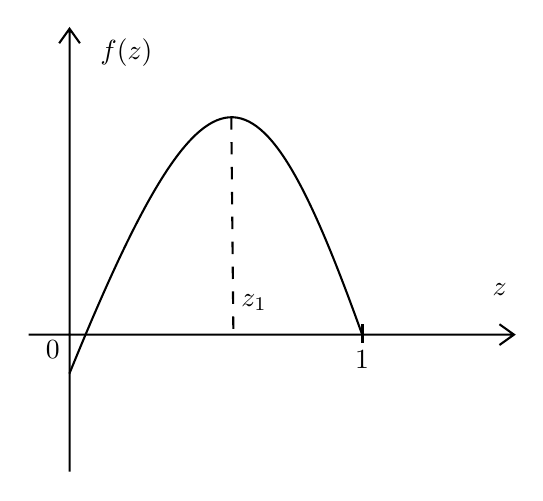
\begin{tikzpicture}[x=0.75pt,y=0.75pt,yscale=-1,xscale=1]
%uncomment if require: \path (0,224); %set diagram left start at 0, and has height of 224

%Shape: Axis 2D [id:dp3848023916381422] 
\draw  (-0.8,148.39) -- (233,148.39)(18.87,1) -- (18.87,214.39) (226,143.39) -- (233,148.39) -- (226,153.39) (13.87,8) -- (18.87,1) -- (23.87,8)  ;
%Straight Lines [id:da9544343505124924] 
\draw    (160,143.39) -- (160,152.39) ;
%Curve Lines [id:da8336123543275722] 
\draw    (18.8,167.19) .. controls (85.8,2.59) and (109.8,8.59) .. (160,148.77) ;
%Straight Lines [id:da3631657909407009] 
\draw  [dash pattern={on 4.5pt off 4.5pt}]  (96.8,43.59) -- (97.8,147.59) ;

% Text Node
\draw (155,154.79) node [anchor=north west][inner sep=0.75pt]    {$1$};
% Text Node
\draw (6,149.79) node [anchor=north west][inner sep=0.75pt]    {$0$};
% Text Node
\draw (100.2,127.4) node [anchor=north west][inner sep=0.75pt]    {$z_{1}$};
% Text Node
\draw (32.2,4.4) node [anchor=north west][inner sep=0.75pt]    {$f( z)$};
% Text Node
\draw (221.2,122.4) node [anchor=north west][inner sep=0.75pt]    {$z$};
\end{tikzpicture}

Пусть сначала $\displaystyle f( 0) =0-\phi _{\xi }( 0) =0\Rightarrow P( \xi =0) =0\Rightarrow q=0$, и существует единственный корень $\displaystyle z_{0} =0$ на $\displaystyle [ 0,\ 1]$. Теперь пусть $\displaystyle f( 0) < 0\Rightarrow P( \xi =0)  >0\Rightarrow \exists !\ z_{0} \in ( 0,\ z_{1}) :\ f( z_{0}) =0$. Заметим, что $\displaystyle f( z) < 0\Leftrightarrow z< z_{0}$.

Покажем, что $\displaystyle q=z_{0}$. Для этого докажем, что $\displaystyle \forall n\in \mathbb{N} \hookrightarrow q_{n} < z_{0}$.

\begin{gather*}
q_{n} =P( X_{n} =0) =P( X_{n-1} =0) +P( X_{n} =0,\ X_{n-1} \neq 0) =\\
=q_{n-1} +\sum _{k=1}^{\infty } P( X_{n-1} =k) \cdotp P( X_{n} =0\ |\ X_{n-k} =k) =\\
=q_{n-1} +\sum _{k=1}^{\infty } P( X_{n-1} =k) \cdotp ( P( \xi _{k} =0))^{k}  >q_{n-1} ,
\end{gather*}
т.к. $\displaystyle \exists k:\ P( X_{n-1} =k) \neq 0$. Далее,
\begin{equation*}
q_{n} =P( X_{n} =0) =\phi _{X_{n}}( 0) =\phi _{\xi }( \phi _{X_{n-1}}( 0)) =\phi _{\xi }( q_{n-1}) < \phi _{\xi }( q_{n}) ,
\end{equation*}
т.к. $\displaystyle \phi _{\xi }$ строго возрастает. Получили, что
\begin{equation*}
f( q_{n}) =q_{n} -\phi _{\xi }( q_{n}) < 0\Rightarrow q_{n} < z_{0} \Rightarrow q=\lim _{n\rightarrow \infty } q_{n} \leqslant z_{0} \Rightarrow q=z_{0} .
\end{equation*}
\end{proof}
\begin{corollary}
Вероятность вырождения -- наименьший корень уравнения $\displaystyle z=\phi _{\xi }( z)$ на $\displaystyle [ 0,\ 1]$.
\end{corollary}